\chapter{Implementation and Verification}\label{ch:implementation}
%From the start of this thesis to the start of this chapter a motivation behind investigation the identification of sources from EEG measurement with more sources than sensors as been exploit. From a linear multiple measurement vector (MMV) model
%\begin{align*}
%\mathbf{Y} = \mathbf{AX},
%\end{align*}
%theory and methods behind recovering the mixing matrix $\mathbf{A}$ and the source matrix $\mathbf{X}$ have been investigated and researched. This lead to two algorithms -- covariance-domain dictionary learning (Cov-DL) algorithm and multiple sparse Bayesian learning (M-SBL) algorithm -- which recover a mixing matrix and a source matrix from the EEG measurements with more sources than sensors, $N > M$.
This chapter describes the implementation process of the baseline algorithm, where the two algorithms Cov-DL and M-SBL resulting from respectively chapter \ref{ch:Cov-DL} and \ref{ch:M-SBL} are implemented and combined into one algorithm.

The implementation of each algorithm is initially tested on a simple simulated data set to verify the implementation. Next, both algorithms are tested on simulated data which aim to resemble real EEG measurements. By simulating the data set the true model parameters are known which allows for measuring the precision of the algorithms, based on a described error measurement.     
In addition different model variables are investigated in order to improve the model.
Finally, the full baseline algorithm is tested on the simulated data and a conclusion is made based on the results. 
%The goal of this chapter is to describe how the two found algorithms can be implemented into one algorithm -- the baseline algorithm -- and what one must have in mind when combining the two algorithms. Furthermore, some tests of the baseline algorithm, with different data sets of different type of data, will be performed with the purpose to investigate how good the recovering process is. 
%The chapter will begin with a discussion of the choice for the parameters $M$, $N$ and $k$ as in the realistic case with real EEG measurements the number of active sources within the brain $k$ are unknown -- which parameters lead to a good recovering?


\section{Algorithm Implementation}
\todo[inline]{ Beskrivelse mangler og flowchart skal opdateres, bl.a. mht. input, som jo er givet fra data}

\begin{enumerate}
\item Introduction to the section
\item Insert the flow diagram and describe how the two algorithm are connected.
\item Perhaps end the section with some description of the complexity of the code.
\end{enumerate}

\begin{figure}[H]
\centering
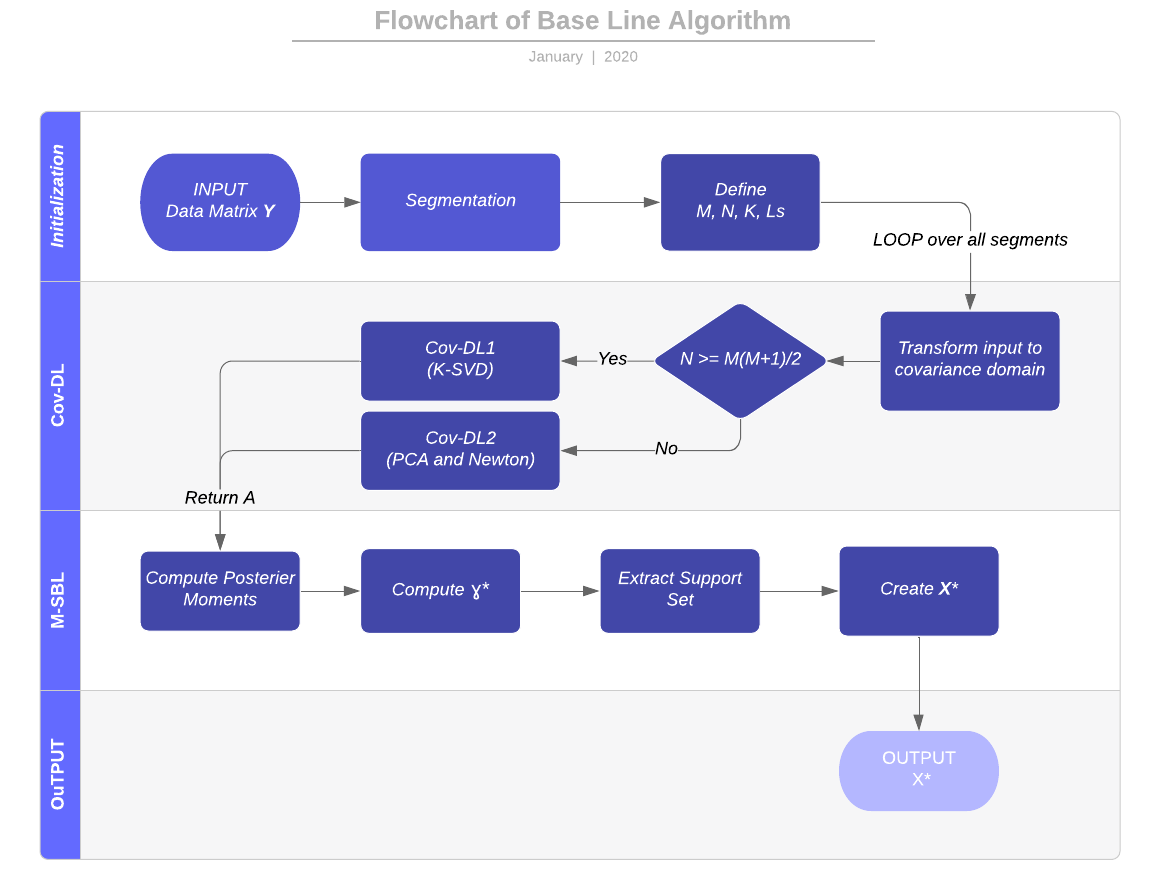
\includegraphics[scale=0.5]{figures/chapter6/Flowchart.png}
\label{fig:flow}
\caption{.}
\end{figure}
\noindent


\section{Data Simulation}\label{sec:dataset}
To evaluate the performance of the main algorithm as well as the individual stages, synthetic data are simulated with respect to the model $\mathbf{Y} = \mathbf{A}\mathbf{X}$. All data sets are simulated based on the following approach, satisfying the sufficient conditions for recovery, displayed in theorem \ref{th:conditions}.
 
A source matrix $\mathbf{X} \in \mathbb{R}^{N \times L}$ is constructed, such that every non-zero row is sampled individually by some function restricted by having zero mean. By this approach the non-zero rows of $\mathbf{X}$ become close to orthogonal \cite{Balkan2014}, which approximates the first conditions of theorem \ref{th:conditions}.   
Then a mixing matrix $\mathbf{A} \in \mathbb{R}^{M \times N}$ is constructed with identically distributed and independent entries. 
As such the source signals are randomly mixed and the mixing matrix fulfils the second condition of theorem \ref{th:conditions}.
With known $\mathbf{A}$ and $\mathbf{X}$, the measurement matrix $\mathbf{Y} \in \mathbb{R}^{M \times L}$ is simulated according to the model, by the matrix product $\mathbf{Y} = \mathbf{AX}$. Note that the error matrix $\mathbf{E}$ is omitted in this chapter, as noise is not included in the synthetic data.  

Two different kinds of data sets are simulated.
Deterministic data having simple and predictable source signals to ensure a solution and easy visualization.
And stochastic data having randomized and fluctuating source signals to resemble realistic EEG measurements.

Note that each simulated data set fulfils the sufficient conditions for recovery, thus segmentation of the synthetic data is not necessary. 

\subsection{Deterministic Data}\label{subseg_simpledata}
Two different deterministic data sets are simulated, with a different number of zero rows. 
The first is specified by $N = 5$, $k = 4$, $M = 3$ and $L = 1000$. 
That is a source matrix $\mathbf{X}$ with $4$ rows individually generated and $1$ zero row. By the specifications the source matrix $\mathbf{X}$ is mixed into a measurement matrix $\mathbf{Y}$ with $3$ measurements per sample.  
The second deterministic data set is specified by $N = 8$, $k = 4$, $M = 3$ and $L = 1000$. 
That is 3 additional zero rows.
From the specifications the first data set comply to $N \leq \widetilde{M}$ which imply the use of Cov-DL2.
The second data set comply to $N > \widetilde{M}$ and $k \leq \widetilde{M}$ implying the use of Cov-DL1. 
As such it is possible to test both branches of the Cov-DL method. 
     
The four non-zero source signals of $\mathbf{X}$ are defined by the following individual functions, causing the rows to be approximately orthogonal
\begin{itemize}
\item[1.] a sinus signal $\sin(2t)$
\item[2.] a sawtooth signal with period $2 \pi t$
\item[3.] a sinus signal $\sin(4t)$
\item[4.] a sign function of a sinus signal $\sin(3t)$
\end{itemize}
with $t$ being a time index defined in the interval $[0,4]$ with $L$ samples. 
Each of the four signals are randomly drawn and used to construct a source matrix $\mathbf{X}$ of size $k \times L$, then zero rows are inserted randomly, such that $\mathbf{X} \in \mathbb{R}^{N \times L}$. 
The mixing matrix $\mathbf{A}$ of size $M \times N$ is randomly generated from a Gaussian distribution. 
By multiplying the source matrix and the mixing matrix a measurement matrix $\mathbf{Y}$ is simulated.
The resulting deterministic data set then consist of $\{ \mathbf{Y}, \mathbf{X}, \mathbf{A} \}$.

In figure \ref{fig:simple} the first deterministic data set, triggering Cov-DL2, is illustrated by the source signals plotted in the top and the measurement signals plotted in the bottom. 
This illustrates how the source signals are transformed by the mixing matrix $\mathbf{A}$.
\begin{figure}[H]
\centering
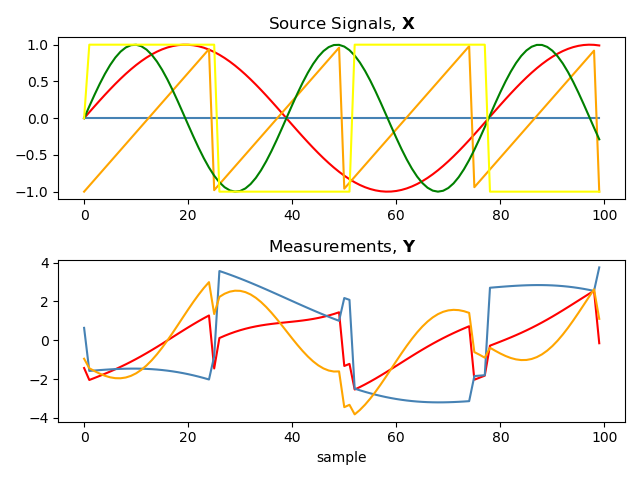
\includegraphics[scale=0.5]{figures/ch_6/simple_data.png}
\caption{Visualization of the source signals $\mathbf{X}$ in comparison to the measurement signals $\mathbf{Y}$ from the deterministic data set specified by $N = 5, M = 3$, $k = 4$ and $L=1000$.}
\label{fig:simple}
\end{figure}
\noindent

\subsection{Stochastic Data}\label{sec:stoch_data}
The purpose of this second kind of data is to resemble EEG measurements for which the main algorithm is intended. 
Here different data sets are simulated depending on the chosen specifications of $N$, $k$, $M$ and $L$. 
Every data set is constructed based on four different linear auto-regressive processes of various orders, each process representing one source signal
\begin{align*}
&x_{t}^{1} = \sum_{i=1}^{2} \phi_i x_{t-i}^{1} + w_t^{1} &x_{t}^{2} = \sum_{i=1}^{2} \zeta_i x_{t-i}^{2} + w_t^{2} \\
&x_{t}^{3} = \sum_{i=1}^{3} \eta_i x_{t-i}^{3} + w_t^{3}  &x_{t}^{4} = \sum_{i=1}^{4} \xi_i x_{t-i}^{4} + w_t^{4}
\end{align*}
%\begin{itemize}
%\item[-] $x_{t}^{1} = \sum_{i=1}^{2} \phi_i x_{t-i}^{1} + w_t^{1}$
%\item[-] $x_{t}^{2} = \sum_{i=1}^{2} \zeta_i x_{t-i}^{2} + w_t^{2}$
%\item[-] $x_{t}^{3} = \sum_{i=1}^{3} \eta_i x_{t-i}^{3} + w_t^{3}$
%\item[-] $x_{t}^{4} = \sum_{i=1}^{4} \xi_i x_{t-i}^{4} + w_t^{4}$
%\end{itemize}
where $\boldsymbol{\phi}, \boldsymbol{\zeta}, \boldsymbol{\eta}$ and $\boldsymbol{\xi}$ are different model parameters and $w_t^{j}$ for $j = 1,\dots ,4$ are mutually independent Gaussian distributed white noise coefficients.
The source matrix $\mathbf{X}$ is constructed by drawing $k$ auto-regressive processes, randomly drawn among the four, each of length $L$. 
If $k < N$ zero rows are inserted randomly such that $\mathbf{X} \in \mathbb{R}^{N \times L}$. 
The mixing matrix $\mathbf{A} \in \mathbb{R}^{M \times N}$ is, like previously, generated randomly from a Gaussian distribution.
By multiplying the source matrix and the mixing matrix, the measurement matrix $\mathbf{Y}$ is simulated. 
The stochastic data set then consist of $\{ \mathbf{Y}, \mathbf{X}, \mathbf{A} \}$. 

One simulation of a stochastic data set is illustrated in figure \ref{fig:AR}. 
The illustrated data set is specified by $N = 5$, $M = 3$, $k = 4$ and $L = 1000$.
\begin{figure}[H]
\centering
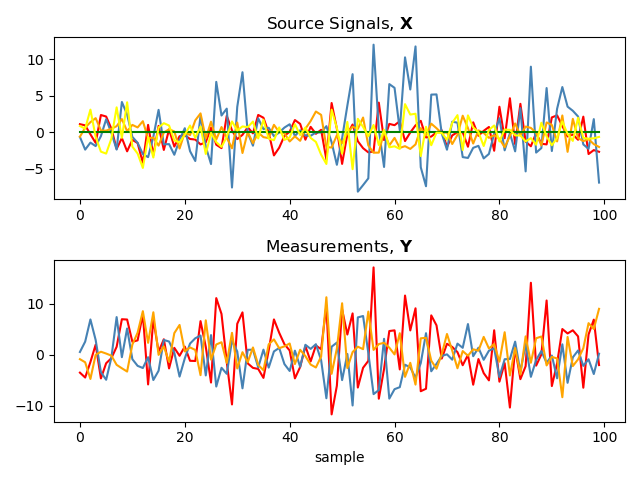
\includegraphics[scale=0.5]{figures/ch_6/AR_data.png}
\caption{Visualization of the source signals $\mathbf{X}$ in comparison to the measurement signals $\mathbf{Y}$ from a stochastic data set specified by $N = 5$, $M = 3$, $k = 4$ and $L=1000$. For simplicity only samples from $L = 0, \dots, 100$ are visualized.}
\label{fig:AR}
\end{figure}
\noindent



\subsection{Error Measurement}  
To evaluate performance of the algorithms it is evident to look at the differences between the true and estimated matrices, mixing matrix $\mathbf{A}$ and source matrix $\mathbf{X}$ -- which is possible due to the input data being simulated. 
For this task the mean squared error (MSE) has been chosen. 
The MSE measures the average squared difference between some estimated value and the true value. 
For $hat{\textbf{g}}$ being the estimate of $\textbf{g}$ the MSE can be written as 
\begin{align*}
\text{MSE}(\textbf{g},\hat{\textbf{g}}) = \frac{1}{T} \sum_{i=1}^T (g_i - \hat{g}_i)^2,  
\end{align*}
with $T$ being the number of elements in the vector $\textbf{g}$. 
In the present case the estimates form a matrix. Here the MSE is computed for each row, which for $\textbf{X}$ is the estimate of one source signal, then the  resulting MSE is the average over all rows. For $\textbf{X}, \hat{\textbf{X}}\in\mathbb{R}^{N\times L}$ the MSE is written as 
\begin{align*}
\text{MSE}(\textbf{X},\hat{\textbf{X}}) = \frac{1}{N} \sum_{i}^{N} \left( \frac{1}{L} \sum_{j=1}^L (\textbf{X}_{ij} - \hat{\textbf{X}}_{ij})^2\right).  
\end{align*}
Similarly, the MSE can be written for $\textbf{A},\hat{\textbf{A}}\in \mathbb{R}^{M \times N}$.  
The MSE is viewed as a measure of the quality of an estimator, in this case of how M-SBL and Cov-DL perform. 
For a large MSE the estimated values are dispersed widely around its mean while for a small MSE value the estimated matrix/values is closely dispersed around the mean. 
Usually, a small MSE value indicates a good estimator but the value cannot be to small as this would indicate that the data has been overfitted \todo{Vi skal lige finde en god kilde som siger dette}. 
Therefore, a good MSE and therefore a good performance would be depending on how the data is scattered as widely scattered data may lead to a MSE value not close to zero but it would still be the a good measure for the estimator.
\todo[inline]{MSE:måske dette kan uddybes lidt i forhold til hvordan vores målingere opføre sig, ved vi hvad vi kan forvente}

   
\section{Algorithm verification}
In this section the implementation of Cov-DL and M-SBL are verified separately based on the MSE between the true- and the estimated model parameters.
During the tests on synthetic data sets the segmentation stage is ignored by letting the simulated data form one single segment.    

\subsection{Test of COV-DL}
As seen from the flow diagram figure \ref{fig:flow} COV-DL takes a measurement matrix $\textbf{Y}$, $N$ and $k$ as input and return an estimation $\hat{\textbf{A}}$ of the mixing matrix $\textbf{A}$. The COV-DL algorithm is tested on the two simulations of the deterministic data, specified in section \ref{subseg_simpledata}. 

\subsubsection{COV-DL1}
For $\textbf{Y}$ specified by $N > \widetilde{M}$ and $k\leq \widetilde{M}$, implying COV-DL1, the true and estimated values of $\textbf{A}$ are plotted in figure \ref{fig:cov1_simple} for visual comparison. Note that each matrix is vectorised such that the corresponding entries are compared.  
The resulting $MSE_{A}$ between the true $\textbf{A}$ and the estimated $\hat{\textbf{A}}$ become 
\begin{align*}
MSE_{A} = 1.37
\end{align*}
From figure \ref{fig:cov1_simple} it is seen that the precision of the estimate varies significant for each entry. Though, values within the a similar range are obtained furthermore the $MSE_{A}$ is fairly small suggesting that the estimate is acceptable\todo[inline]{how should we determined this?? and can we give an explanation. \\
jeg har kigget nærmere på dictionary learning funktionen, jeg kan ikke ændre på resultater ved at ændre på k, den er som standard sat til 0.1*n, hvilket er langt mere sparse (under 1 non-zero) end vores system. med ved algorithm ='lars' skulle den godtage k, som ellers for 'omg' bliver overskrevet at standarden. \\
for at undersøge om det igen kan være forholdet mellem A og D, har jeg lavet et system med N=16, M=5, k=4, som skal kunne løsese med dictionary lerning uden brug af covariance domænet. dog bliver resultatet ikke bedre. uanset input så falder A(estimate) altid inden for [-1,1], hvilket er et problem.}  

\subsubsection{COV-DL2}
For $\textbf{Y}$ specified by $N\leq \widetilde{M}$, implying Cov-DL2, the true and estimated values of $\textbf{A}$ are plotted in figure \ref{fig:cov2_simple} for visual comparison. Additionally, is the initial $\textbf{A}$ plotted in the same figure, as standard that is a Gaussian matrix $\textbf{A}_{init}$ which is given to the optimization solver within COV-DL2.    
The resulting $MSE_{A}$ between the true $\textbf{A}$ and the estimated $\hat{\textbf{A}}$ become 
\begin{align*}
MSE_{A} = 2.46 
\end{align*}
From figure \ref{fig:cov2_simple} the estimate $\hat{\textbf{A}}$ shows visual tendencies from the true $\textbf{A}$. However, when it is compared to the initial guess of $\textbf{A}$ it is seen that the resulting estimate have moved further away from the true $\textbf{A}$ compared to $\textbf{A}_{init}$. this suggest some flaw within the optimization process. By printing the convergence message from the used optimization solver it is confirmed that the optimization process was found to be terminated successful. With current function value at $0.0$ after 26 iterations. 
With the resulting cost at 0.0 this suggest that an global minima has been found, but this minima do not correspond to the true $\textbf{A}$.    
To confirm this the following evaluations of the cost function was conducted. 
\begin{align*}
&\text{cost}(\hat{\textbf{A}}) = 0.0\\
&\text{cost}(\textbf{A}_{init}) = 1.564\\
&\text{cost}(\textbf{A}) = 1.809
\end{align*}
These evaluations ensures that the optimization solver have manage to find the solution that minimizes the cost function. By evaluating the cost function with respect to the true $\textbf{A}$ is it seen that it is not a global minimizer to the optimization problem. This suggest that the optimization problem, derived in section \ref{sec:over_det}, do not fulfil the purpose\todo{what word to use here? Jan brugte diverger om noget?}    

\begin{figure}[h]
    \begin{minipage}[t]{.45\textwidth}
		\centering
		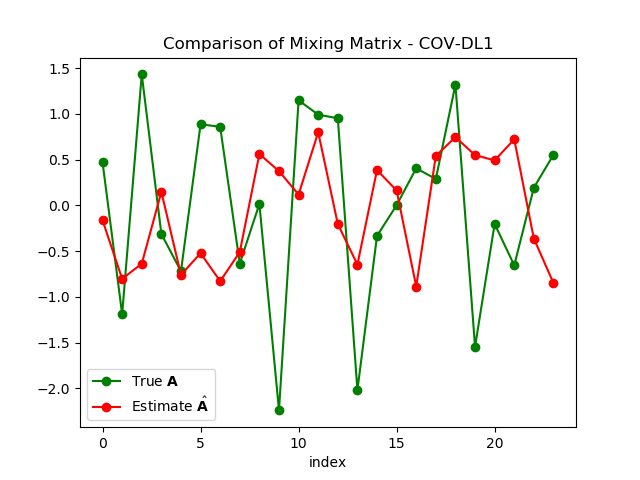
\includegraphics[scale=0.5]{figures/ch_6/COV1_simple.png}
		\caption{Estimated values of $\hat{\textbf{A}}$ compared to the true 				values $\textbf{A}$}
		\label{fig:cov1_simple}
    \end{minipage} 
    \hfill
    \begin{minipage}[t]{.45\textwidth}
        \centering
		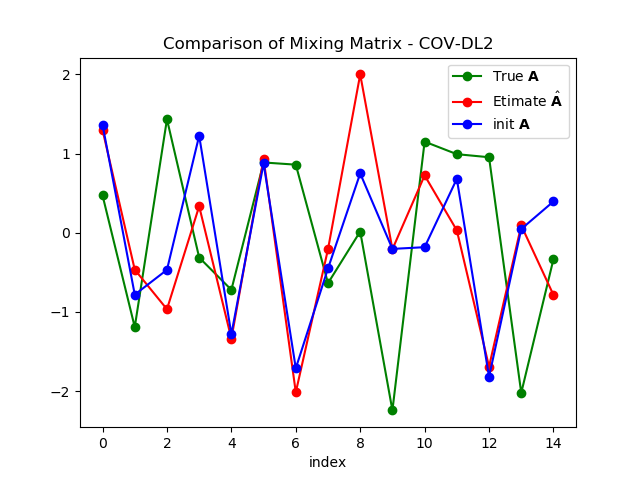
\includegraphics[scale=0.5]{figures/ch_6/COV2_simple.png}
		\caption{The initial $\textbf{A}$ and the estimate $\hat{\textbf{A}}$ 				compared to the true values $\textbf{A}$. }
		\label{fig:cov2_simple}
    \end{minipage}
\end{figure}

\subsubsection{Conclusion to $\hat{\textbf{A}}$}
From the above results is it found that the estimate $\hat{\textbf{A}}$, especially within the COV-DL2 branch, can not be consider a valid estimate of the mixing matrix $\textbf{A}$. It is suggested that the flaw lies within either the  derivation of the optimization problem, more specifically within the assumption made throughout the derivation concerning the relation between $\textbf{A}, \textbf{D}$ and $\textbf{U}$. This statement build upon the success of the(non documented) unit tests of the COV-DL2 algorithm suggesting that the optimisation of D not depending on A is possible(?eller hvad var det vi gjorde?)...
The appearance of this issue may suggest that there is a lack within the published results \cite{Balkan2015}(?tjek)considering the possibility of reconstructing the results.  

Due to the time limitation of the project the error is not investigated further, and it is concluded that the estimate of $\textbf{A}$ is not valid hence it will not be used as an input for the next stage of the algorithm, M-SBL. 

This conclusion suggest that an alternative action must be considered. This is discussed further in section \ref{sec:est_base}

        

\subsection{Alternative to $\hat{\textbf{A}}$}

\subsection{Test of M-SBL}
From the flow diagram figure \ref{fig:flow} it seen that that the M-SBL algorithm takes $\mathbf{A}$ (maybe $k$) and $\mathbf{Y}$ as input. The algorithm is now tested on the same two simple data sets specified by $M = 3$, $k = 4$, $L=1000$ and respectively $N = 5$ and $N = 8$ as used above. 
In order to not let the performance of Cov-DL affect the result of M-SBL it is the true $\mathbf{A}$ which is given as input along with the corresponding $\mathbf{Y}$. The estimate $\hat{\mathbf{X}}$ are plotted in figure \ref{fig:M-SBL_simple1} and \ref{fig:M-SBL_simple2}. Each non-zero signals are now plotted separately for simple visual comparison. Furthermore, note that each compared couple of rows have the same row index, as such the localization of the estimated row can be evaluated.
\begin{figure}[H]
    \begin{minipage}[t]{.45\textwidth}
    	\centering
		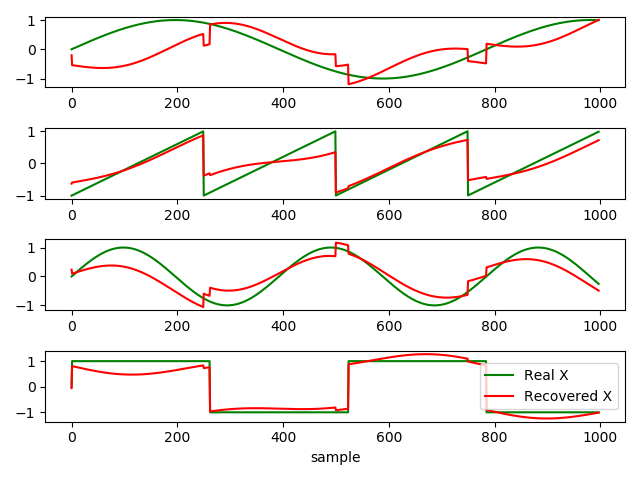
\includegraphics[scale=0.5]{figures/ch_6/M-SBL_simple1.png}
		\caption{Estimated values of $\hat{\textbf{X}}$ compared to the true 					values $\textbf{X}$. From measurement $\textbf{Y}$ specified by $N=5$, $M = 3$, $k=4$ and $L=1000$}
		\label{fig:M-SBL_simple1}
    \end{minipage} 
    \hfill
    \begin{minipage}[t]{.45\textwidth}
        \centering
		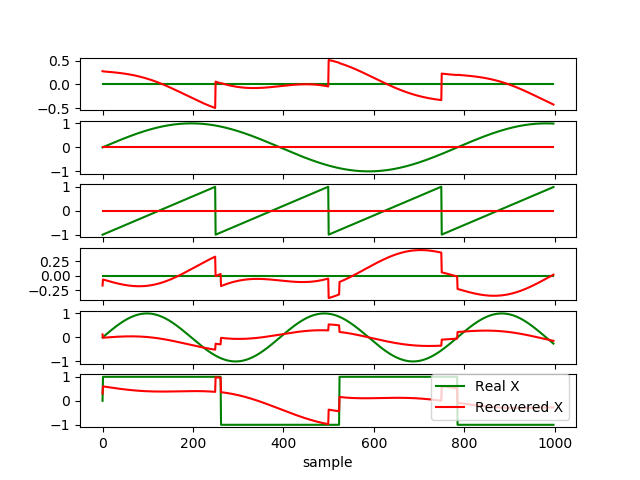
\includegraphics[scale=0.5]{figures/ch_6/M-SBL_simple2.png}
		\caption{Estimated values of $\hat{\textbf{X}}$ compared to the true 				values $\textbf{X}$. From measurement $\textbf{Y}$ specified by $N=8$, $M = 3$, $k=4$ and $L=1000$ }
		\label{fig:M-SBL_simple2}
    \end{minipage}
\end{figure}
The resulting MSE between the true $\textbf{X}$ and the estimated $\hat{\textbf{X}}$ from figure \ref{fig:M-SBL_simple1} where $N = 5$, averaged over every row, become 
\begin{align*}
X_{MSE} = 0.131 
\end{align*}
From figure \ref{fig:M-SBL_simple1} it is seen that all four source signals are recovered at the right location. As suggested by the achieved MSE it the estimates are not exact, but it is clear that the estimates manage to follow the right pattern at the right location. By this plot an error margin are established(?).  

The resulting MSE between the true $\textbf{X}$ and the estimated $\hat{\textbf{X}}$ from figure \ref{fig:M-SBL_simple2} where $N = 8$ thus more sparse, become 
\begin{align*}
X_{MSE} = 0.145 
\end{align*}
From figure \ref{fig:M-SBL_simple2} it is seen that first source signal are recovered at the third entry, that is one dislocation, while the rest are recovered at the right location. This indicate that the algorithm can manage to locate the source signal however the more options the more greater chance of dislocation.     

\subsubsection*{Possibilities of $N=k$}
\begin{itemize}
	\item The true $N$ is unknown for real EEG measurements, as it change for every brain
	\item Therefore, we do not know the amount of activation inside the brain, but it is those which are of interest in this thesis.
	\item Due to the method for determine the mixing matrix $\textbf{A}$ the ration between $N$ and $k$ do not affect the result, hence there are no argument against letting $N=k$ which will lower the computational complexity.\todo[inline]{do the same argument regarding $N=k$ hold for the determination of $\textbf{X}$? after the awareness that we do not need to provide $k$ to M-SBL as it has been done so far.}    
\end{itemize}

\section{Test on AR data and model fitting}
The implemented algorithms are now tested on the simulated autoregressive data sets which resembles the real EEG measurements. Furthermore it is sought to improve the model by fitting specific model variables to the data. In this case it is the Cov-DL algorithm which can be adjusted for the overdetermined case where Cov-DL2 is used.      

\subsection{Model Fitting}
Two model variables are now considered with the purpose of improving the performance of the COV-DL algorithm. The initial A given to the optimization problem \eqref{eq:Cov_DL2} within COV-DL2, and the segmentation size used within the covariance domain.   
\subsubsection*{Initial $\textbf{A}$}
Consider the COV-DL algorithm in the case where the system transformed into the covariance domain results in an overdetermined system. In this case the COV-DL2 branch of the algorithm is used. 
When estimating the mixing matrix $\mathbf{A}$ a matrix $\mathbf{D}$ is used in the process. For the over-determined system \ref{sec:over_det} $\mathbf{D}$ is found by solving the optimisation problem \eqref{eq:Cov_DL2} with respect to $\hat{\textbf{A}}$. To solve the optimization problem an initial $\mathbf{A}_{\text{ini}}$ is given. The choice of this initial $\mathbf{A}_{\text{ini}}$ may affect how the good an estimate the recovered mixing matrix $\mathbf{A}$ is.
Three different choices of $\mathbf{A}_{\text{ini}}$ are considered:
\begin{itemize}
\item[-] A matrix $\mathbf{A1}$ drawn from a continuous uniform distribution in the half-open interval $[0.0, 1.0)$
\item[-] A matrix $\mathbf{A2}$ drawn from a uniform distribution in the half-open interval $[-1.0, 1.0)$
\item[-] A matrix $\mathbf{A3}$ drawn from a Gaussian distribution with mean 0 and variance 1
\end{itemize}
The test of different initial $\mathbf{A}_{\text{ini}}$ is performed on the 
an AR data set specified by $N=5$ $M = 3$, $k = 4$ and $L = 1000$. 
The MSE of the three tests are seen in table \ref{tab:iniA} 
\begin{table}[H]
\centering
\begin{tabular}{|l|l|l|l|} 
\hline
                          & \textbf{A1} & \textbf{A2} & \textbf{A3} \\
\hline $\text{MSE}_{\mathbf{A}}$ &   2.15          & 2.00            & 1.88\\
\hline           
\end{tabular}
\caption{Resulting MSE for varying initial A, used within COV-DL2.}
\label{tab:iniA}
\end{table}
\todo[inline]{is it okay that we do not include the mse of X here, I don't think is any reasoning to do it, but it should be check later whether the error of A follows the error of X as it is asumped at this moment.}
From the results it is seen that \textbf{A3} achieves the lowest MSE, thus an Gaussian distributed initial $\textbf{A}$ will be used.    
 
% old results
%For the test we are looking at a system of size $M = 8$, $k = 16$ and $L = 1000$. Furthermore, for the Cov-DL the data has been divided in segments of 10 samples leading to 100 segments.
%\begin{figure}[H]
%\centering
%    \begin{minipage}[t]{.45\textwidth}
%        \centering
%		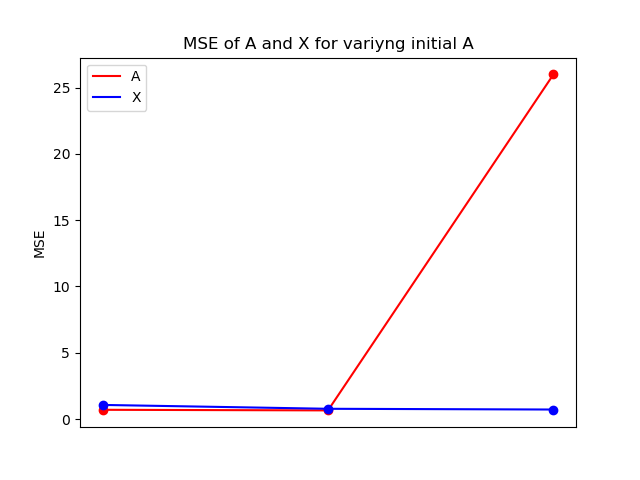
\includegraphics[scale=0.5]{figures/chapter6/Mix_Error_initial_A_m8_k16_L1000.png}
%		\subcaption{Simple Data Set - Estimated A}
%    \end{minipage} 
%    \hfill
%    \begin{minipage}[t]{.45\textwidth}
%        \centering
%		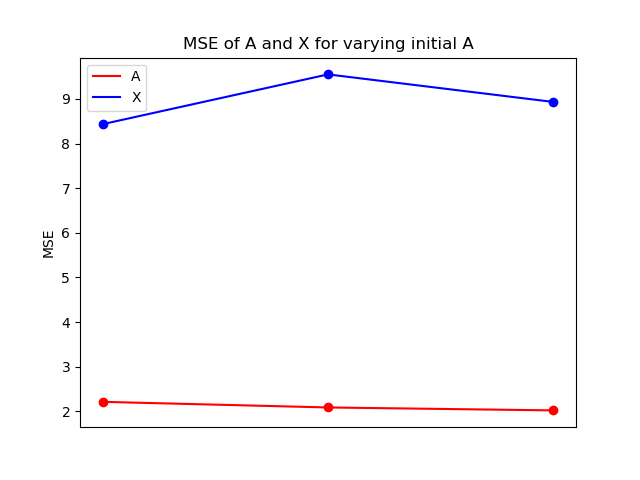
\includegraphics[scale=0.5]{figures/chapter6/AR_Error_initial_A_m8_k16_L1000.png}
%		\subcaption{Autoregressive Data Set - Estimated A}
%    \end{minipage}
%    \begin{minipage}[t]{.45\textwidth}
%        \centering
%		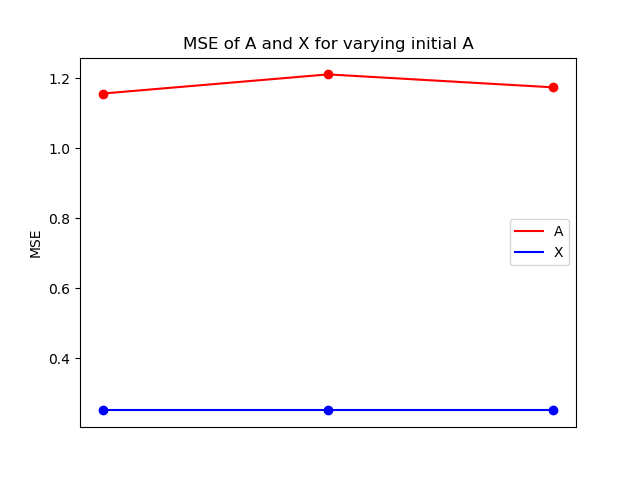
\includegraphics[scale=0.5]{figures/chapter6/Mix_Error_initial_A_m8_k16_L1000_RealA.png}
%		\subcaption{Simple Data Set - Real A}
%    \end{minipage} 
%    \hfill
%    \begin{minipage}[t]{.45\textwidth}
%        \centering
%		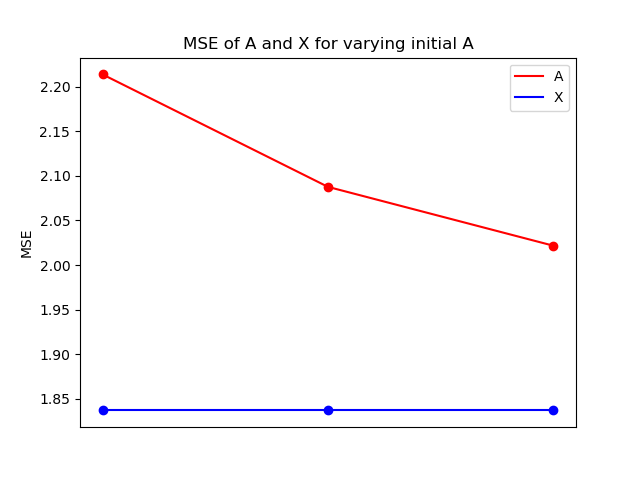
\includegraphics[scale=0.5]{figures/chapter6/AR_Error_initial_A_m8_k16_L1000_RealA.png}
%		\subcaption{Autoregressive Data Set - Real A}
%    \end{minipage}
%\caption{}
%\label{fig:initialA}
%\end{figure}
%\noindent
%The MSE values of each tests -- estimated and real mixing matrix $\mathbf{A}$ -- can be seen in table \ref{tab:iniA}. For the real mixing matrix the MSE values of source matrix $\mathbf{X}$ are identical because the real mixing matrix is not influenced by the three different initial $\mathbf{A}_{\text{ini}}$.
%\begin{table}[H]
%\begin{minipage}{.5\linewidth}
%\centering
%\begin{tabular}{|c|c|c|c|}
%\hline 
% & $\mathbf{A1}$ & $\mathbf{A2}$ & $\mathbf{A3}$ \\ 
%\hline 
%MSE of $\mathbf{A}$ & 1.16 & 1.21 & 1.17 \\ 
%\hline 
%MSE of $\mathbf{X}$ & 0.69 & 0.66 & 0.81 \\ 
%\hline 
%\end{tabular} 
%\subcaption{Simple Data Set - estimated $\mathbf{A}$}
%\end{minipage}
%\begin{minipage}{.5\linewidth}
%\centering
%\begin{tabular}{|c|c|c|c|}
%\hline
% & $\mathbf{A1}$ & $\mathbf{A2}$ & $\mathbf{A3}$ \\ 
%\hline 
%MSE of $\mathbf{A}$ & 2.21 & 2.09 & 2.02 \\ 
%\hline 
%MSE of $\mathbf{X}$ & 8.43 & 9.55 & 8.93 \\ 
%\hline
%\end{tabular} 
%\subcaption{Autoregressive Data Set - estimated $\mathbf{A}$}
%\end{minipage}
%\begin{minipage}{.5\linewidth}
%\centering
%\begin{tabular}{|c|c|c|c|}
%\hline 
% & $\mathbf{A1}$ & $\mathbf{A2}$ & $\mathbf{A3}$ \\ 
%\hline 
%MSE of $\mathbf{A}$ & $\times$ & $\times$ & $\times$ \\ 
%\hline 
%MSE of $\mathbf{X}$ & 0.25 & 0.25 & 0.25 \\ 
%\hline 
%\end{tabular} 
%\subcaption{Simple Data Set - real $\mathbf{A}$}
%\end{minipage}
%\begin{minipage}{.5\linewidth}
%\centering
%\begin{tabular}{|c|c|c|c|}
%\hline
% & $\mathbf{A1}$ & $\mathbf{A2}$ & $\mathbf{A3}$ \\ 
%\hline 
%MSE of $\mathbf{A}$ & $\times$ & $\times$ & $\times$ \\ 
%\hline 
%MSE of $\mathbf{X}$ & 1.84 & 1.84 & 1.84 \\ 
%\hline
%\end{tabular} 
%\subcaption{Autoregressive Data Set - real $\mathbf{A}$}
%\end{minipage}
%\caption{(a) This are the MSE values achieve from the simple data set and (b) is the MSE values achieved from the autoregressive data set.}
%\label{tab:iniA}
%\end{table}
%\noindent
%From \ref{tab:iniA} we see that the MSE values for our estimated mixing matrix $\mathbf{A}$ are overall small compared to both data sets. However, if we look at the results for the source matrix there are a big different from the simple data set and the autoregressive data set and comparing it to the results with the real mixing matrix. 
%As the autoregressive data set have a higher amplitude in the data than the simple data set, the error will become larger. 
%
%If we look at the initial $\mathbf{A}_{\text{ini}}$ drawn from the Gaussian distribution we have a small error for the mixing matrix in the autoregressive data set while the error from the simple data set also is low. The error for source matrix is the highest value for the simple data set but comes second in the autoregressive data set. As we want to take into account that the autoregressive data set resemble the EEG measurement most we conclude that the initial $\mathbf{A}_{\text{ini}}$ from the Gaussian distribution would be the best choice in Cov-DL.

\subsubsection{Segmentation in Covariance domain}
For the Cov-DL algorithm when estimating the mixing matrix $\mathbf{A}$ the measurement matrix is transformed into the covariance domain as part of the recovering process. During the transformation the measurement matrix $\mathbf{Y}$ is divided into segments consisting of $L_s$ samples each.
During this test different numbers of samples within a segment will be tested to see how this affect the performance of the algorithm.

The autoregressive data sets,  $M = 3$, $k = 4$ and $L = 1000$ samples and with respectively $N = 5$ and $N=8$, will be used for the testing. With $k = 4$ the number of segments can not be less than the number of sources. For this system each segment can have maximum $L_s = 200$ corresponding to minimum 5 segments. 

For the test, six different number of samples within each segments will be tested, $L_s = \{ 10, 20, 30, 50, 100, 150, 200 \}$. Furthermore, each $L_s$ will be run 10 times and the output of the test will be average such that each $L_s$ have one average MSE.
%\begin{figure}[H]
%\centering
%    \begin{minipage}[t]{.45\textwidth}
%        \centering
%		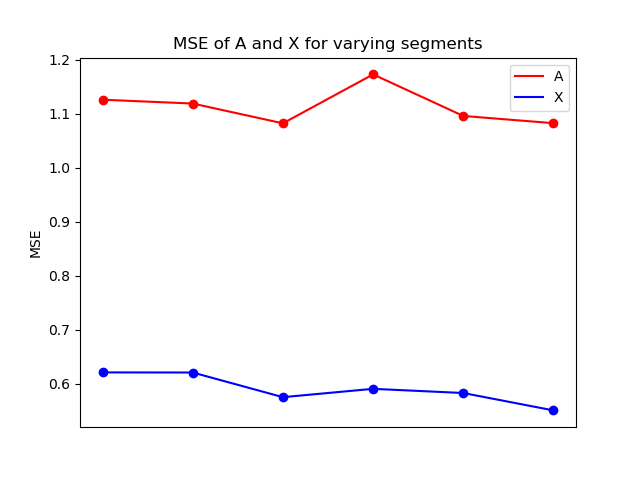
\includegraphics[scale=0.5]{figures/chapter6/Mix_Error_vary_covseg_m8_k16_L1000}
%		\subcaption{Simple Data Set - Estimated A}
%    \end{minipage} 
%    \hfill
%    \begin{minipage}[t]{.45\textwidth}
%        \centering
%		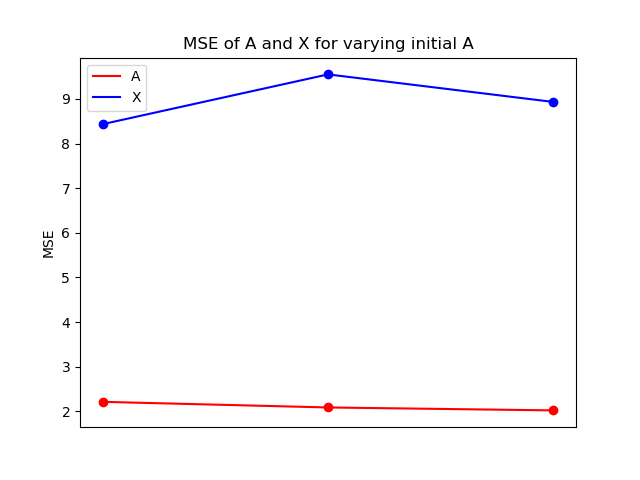
\includegraphics[scale=0.5]{figures/chapter6/AR_Error_initial_A_m8_k16_L1000.png}
%		\subcaption{Autoregressive Data Set - Estimated A}
%    \end{minipage}
%    \begin{minipage}[t]{.45\textwidth}
%        \centering
%		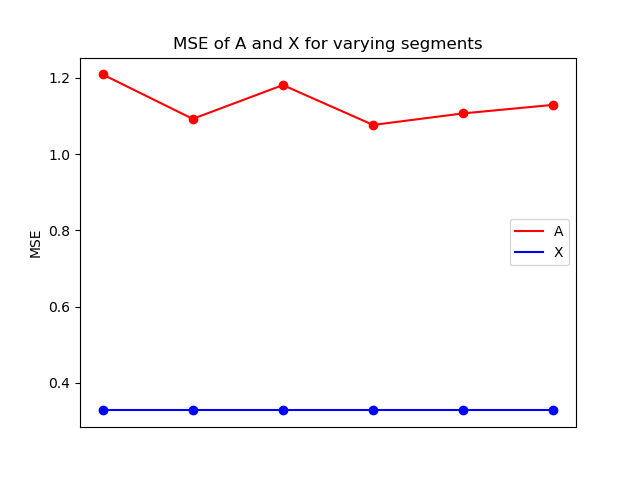
\includegraphics[scale=0.5]{figures/chapter6/Mix_Error_vary_covseg_m8_k16_L1000_RealA.png}
%		\subcaption{Simple Data Set - Real A}
%    \end{minipage} 
%    \hfill
%    \begin{minipage}[t]{.45\textwidth}
%        \centering
%		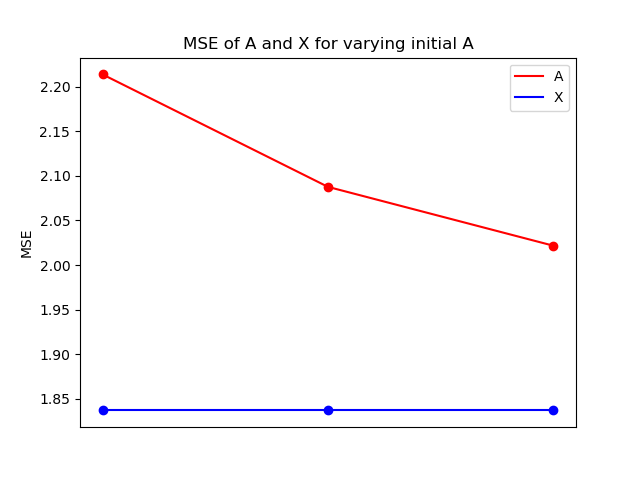
\includegraphics[scale=0.5]{figures/chapter6/AR_Error_initial_A_m8_k16_L1000_RealA.png}
%		\subcaption{Autoregressive Data Set - Real A}
%    \end{minipage}
%\caption{}
%\label{fig:seg}
%\end{figure}
%\noindent
%The MSE values of each tests -- estimated and real mixing matrix $\mathbf{A}$ -- can be seen in table \ref{tab:seg}\todo[inline]{hvordan kan det være der kun er 3 punkter for AR dataen?\\
%\textbf{X} fejlen er mærkelig høj her, er der en grund til det}.

\begin{table}[H]
\centering
\begin{minipage}{.45\textwidth}
\centering
\begin{tabular}{|c|c|c|c|c|c|c|c|}
\hline 
& 10 & 20 & 30 & 50 & 100 & 150 & 200 \\ 
\hline 
Average MSE of $\hat{\mathbf{A}}$ & 1.86 & 2.14 & 2.21 & 2.03 & 2.31 & 1.89 & 2.06 \\ 
\hline
\end{tabular} 
\caption{MSE values from measurement specified by $N=5$, $M = 3$, $k = 4$ and $L = 1000$ achieved from the used of Cov-DL2}
\label{tab:seg1}
\end{minipage}
\\
\begin{minipage}{.45\textwidth}
\centering
\begin{tabular}{|c|c|c|c|c|c|c|c|}
\hline 
& 10 & 20 & 30 & 50 & 100 & 150 & 200 \\ 
\hline 
Average MSE of $\hat{\mathbf{A}}$ & 1.29 & 1.37 & 1.22 & 1.16 & 1.46 & 1.20 & 1.32 \\ 
\hline
\end{tabular} 
\caption{MSE values from measurement specified by $N=8$, $M = 3$, $k = 4$ and $L = 1000$ achieved the used of Cov-DL1.}
\label{tab:seg2}
\end{minipage}
\end{table}
\noindent
Overall, in table \ref{tab:seg1} and \ref{tab:seg2} there is not a big variation between the MSE values of both data sets. One could argument that the number of samples within each segment does not affect the performance of the algorithms as much and therefore is more free choice.

\subsection{Test on AR data}
Both algorithms are now test on AR data set ..... missing description


\begin{figure}[H]
    \begin{minipage}[t]{.45\textwidth}
    	\centering
		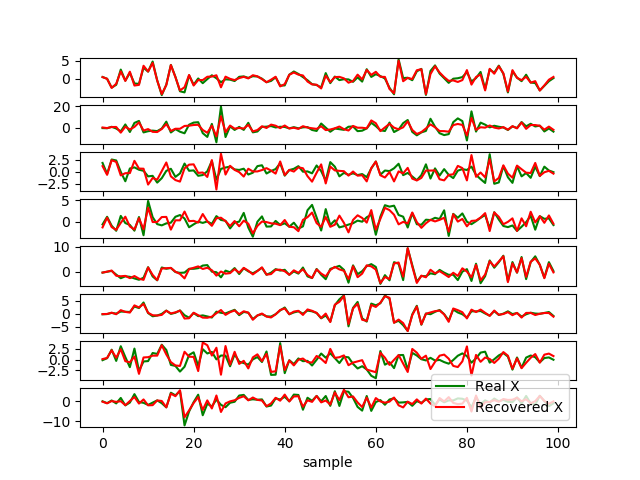
\includegraphics[scale=0.5]{figures/ch_6/M-SBL_AR1.png}
		\caption{ $N=5$, $M = 3$, $k=4$ and $L=1000$  - True $\textbf{A}$}
		\label{fig:AR1}
    \end{minipage} 
    \hfill
    \begin{minipage}[t]{.45\textwidth}
        \centering
		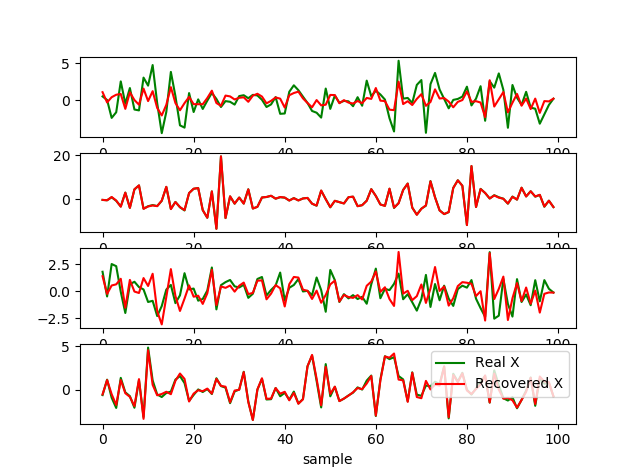
\includegraphics[scale=0.5]{figures/ch_6/M-SBL_AR2.png}
		\caption{$N=k=4$ $M = 3$ and $L=1000$ - True $\textbf{A}$}
		\label{fig:AR2}
    \end{minipage}
\end{figure}


MSE for $N=5$, $k=4$ is 2.17\\
MSE for $N=k=4$ is 0.682\\


 


\section{Test of the Main Algorithm}\label{sec:test_base}
In this section the performance of the main algorithm is tested. That is the algorithm visualised in the flow diagram, figure \ref{fig:flow}, where the COV-DL algorithm and the M-SBL algorithm i combined. However, as dissucsed due to the negative conclusion on the verification of COV-DL an alternative has to be is considered.  
 
\subsection{Alternative to Estimate $\hat{\textbf{A}}$}  
As concluded the Cov-DL algorithm do not recover a sufficient estimate of the mixing matrix $\mathbf{A}$, therefore a different approach is necessary. 

Replacing the insufficient estimate by a fixed estimate $\hat{\mathbf{A}}_{\text{fix}}$ is one immediately solution. 
This choice is supported by the observations from Cov-DL2 where $\mathbf{A}_{\text{ini}}$ matrix provides an estimate which is happens to be a least as good as the one provided by Cov-DL. 
Thus the challenge is now to determine a fixed matrix for which its characteristics resembles those of the true mixing matrix. 
However, from chapter \ref{ch:motivation} it is clear that no specific characteristic of the mixing matrix is known, which supports the choice of an random matrix of Gaussian distribution or similar, as it was chosen for the initial guess $\mathbf{A}_{\text{init}}$ for the estimate.   
From this perspective three fixed mixing matrices are defined, by drawing each entry from a specified distribution: 
\begin{itemize}
\item[] $\hat{\mathbf{A}}_{\text{uni}} \sim \mathcal{U}(-1,1)$
\item[] $\hat{\mathbf{A}}_{\text{norm1}} \sim \mathcal{N}(0,1)$                                           
\item[] $\hat{\mathbf{A}}_{\text{norm2}} \sim \mathcal{N}(0,2)$ 
\end{itemize}
Note that the third matrix $\hat{\mathbf{A}}_{\text{norm1}}$ is generated the same way as the true mixing matrix of the stochastic data sets. 
Thus it is expected to have the lowest MSE when compared to the true mixing matrix $\mathbf{A}$. 
However, it is of interest to investigate whether it is the best estimate of $\mathbf{A}$ which provide the best estimate of $\mathbf{X}$.   

A different option regarding a choice for a fixed $\hat{\mathbf{A}}$ is to utilize the ICA algorithm, described in appendix \ref{app:ICA}. 
By the ICA algorithm it is possible to solve the EEG inverse problem for both $\mathbf{A}$ and $\mathbf{X}$, in the case where $k \leq M$.
Consider a simulation of a stochastic data set specified by $N = k = M$. 
Solving the system by ICA yields an estimate of $\mathbf{A}$. 
Now reduce the data set $\mathbf{Y}$ such that $M \leq k$. 
Similar the estimate of $\mathbf{A}$ is reduced by removing the same rows as in $\mathbf{Y}$, this yields the an estimate $\hat{\mathbf{A}}_{\text{ICA}}$ which can be used as a fixed input to M-SBL along with the corresponding reduced $\mathbf{Y}$.

The four different fixed estimates $\hat{\mathbf{A}}$ are tested on stochastic data sets specified by $M = 10$, $N = k = 16$ and $L = 1000$, where the estimate $\hat{\mathbf{A}}_{\text{ICA}}$ has been reduced to $M = 10$. 
As a reference the $\textbf{A}_{true}$ is included in the plot, to see the best possible $MSE(\textbf{X},\hat{\textbf{X}})$.
To get an average performance 50 different simulations are conducted with the same specifications, each system $\mathbf{X}$ is estimated from each of the four fixed estimates of $\mathbf{A}$\footnote{Note that for each of the 10 repetitions four new $\hat{\mathbf{A}}_{\text{fix}}$ are fixed.}, and the MSE are computed. 
The resulting averaged $\text{MSE}(\mathbf{A}, \hat{\mathbf{A}}_{\text{fix}})$ and $\text{MSE}(\mathbf{X}, \hat{\mathbf{X}})$ are visualised in figure \ref{fig:vary_A}, for each of the four $\hat{\mathbf{A}}_{\text{fix}}$. 
Furthermore, the plotted values are found in table \ref{tab:fixed}.
\begin{figure}[H]
\centering
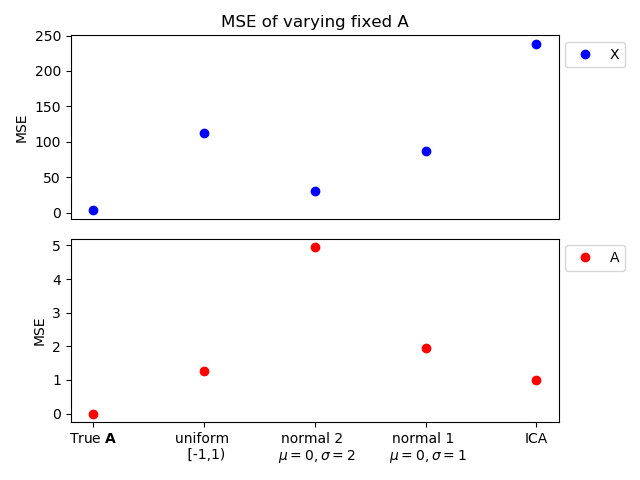
\includegraphics[scale=0.5]{figures/ch_6/A_fix1.png}
\caption{Average MSE values for each of the four fixed mixing matrix $\hat{\mathbf{A}}_{\text{fix}}$ resulting from a stochastic data set specified by $M=10$, $N=k=16$ and $L=1000$.}
\label{fig:vary_A}
\end{figure}
\noindent

\begin{table}[H]
\centering
\begin{tabular}{|c|c|c|c|c|c|}
\hline
 &  $\hat{\mathbf{A}}_{\text{true}}$ & $\hat{\mathbf{A}}_{\text{uni}}$ & $\hat{\mathbf{A}}_{\text{norm2}}$	 & $\hat{\mathbf{A}}_{\text{norm1}}$ & $\hat{\mathbf{A}}_{\text{ICA}}$ \\
\hline
$\text{MSE}(\mathbf{A}, \hat{\mathbf{A}}_{\text{fix}})$ & 0 & 1.271 & 4.957 & 1.941 & 1.006 \\
\hline
$\text{MSE}(\mathbf{X}, \hat{\mathbf{X}})$ & 3.271 & 113.10 & 30.02 & 86.51 & 238.5 \\
\hline
\end{tabular}
\caption{Average MSE values resulting from stochastic data set specified by $M=10$, $N=k=16$ and $L=1000$ with a fixed estimate of the mixing matrix $\hat{\mathbf{A}}_{\text{fix}}$.}
\label{tab:fixed}
\end{table}
\noindent

From table \ref{tab:fixed} and figure \ref{fig:vary_A} it is first of all seen that relation between the MSE of $\textbf{A}$ and $\textbf{X}$ is not as expected, as the lowest $\text{MSE}(\mathbf{A}, \hat{\mathbf{A}}_{\text{fix}})$ results in the highest $\text{MSE}(\mathbf{X}, \hat{\mathbf{X}})$ and so forth. 
The lowest $\text{MSE}(\mathbf{A}, \hat{\mathbf{A}}_{\text{fix}})$ is achieved by using $\hat{\mathbf{A}}_{\text{ICA}}$, which confirms that the ICA algorithm manage to estimate $\mathbf{A}$ when $k \leq M$. 
However, as this do not result in the best estimate of $\mathbf{X}$ a different choice of $\hat{\mathbf{A}}$ is still considered. 
The lowest $\text{MSE}(\mathbf{X}, \hat{\mathbf{X}})$ is achieved by use of $\hat{\mathbf{A}}_{\text{norm}}$, which resulted in the largest $\text{MSE}(\mathbf{A}, \hat{\mathbf{A}}_{\text{fix}})$. 
      
As the main interest in this thesis is to identify and localize the active sources of EEG measurements a low $\text{MSE}(\mathbf{X}, \hat{\mathbf{X}})$ is more desirable than a low $\text{MSE}(\mathbf{A}, \hat{\mathbf{A}}_{\text{fix}})$. 
Furthermore, a disadvantage of using $\hat{\mathbf{A}}_{\text{ICA}}$ is the limitations in practice when $k = M$ is not possible.     
From these observation a fixed estimate of the mixing matrix drawn from a normal distribution with mean 0 and variance 2, $\hat{\mathbf{A}}_{\text{norm}}$, is chosen as the the alternative estimate of $\mathbf{A}$, and is used throughout the thesis. 

Due to the unexpected relation between $MSE(\mathbf{A}, \hat{\mathbf{A}}_{\text{fix}})$ and $\text{MSE}(\mathbf{X}, \hat{\mathbf{X}})$ an additional plot is computed. Figure \ref{fig:X_func_SNR} show the $\text{MSE}(\mathbf{X}, \hat{\mathbf{X}})$ as a function of $\hat{\textbf{A}}$ with varying SNR value. 
Additionally figure \ref{fig:A_func_SNR} show the corresponding MSE between the True $\textbf{A}$ and $\hat{\textbf{A}}$ where an increasing amount of noise is added.
Note that the noise variance is decreasing along the x-axis. 
The noise is generated as Gaussian white noise, with increasing variance corresponding to the desired SNR value. The SNR value is considered in the interval [0.01, 2]. 
From figure \ref{fig:X_func_SNR} it is seen that MSE decreases as the SNR decreases. This indicates as first expected that the better estimate of $\textbf{A}$ the better estimate of $\textbf{X}$. However this is still an contradiction to the result seen in figure \ref{fig:vary_A}. 
This can however be due to the fact that the true $\textbf{A}$ being a Gaussian matrix with $\mu = 0$ and $\sigma = 1$ for which Gaussian noise is added. The MSE between the true $\textbf{A}$ and the noisy $\hat{\textbf{A}}$ seen in figure \ref{fig:A_func_SNR} is not as high as expected due to the relative large amount of noise, all being remarkably less than the corresponding MSE in table \ref{tab:fixed} \todo{det skal tydeliggøres om der er brugt gentagelser her eller er det bare et run. - T}.  


\begin{figure}[H]
    \begin{minipage}[t]{.45\textwidth}
    	\centering
		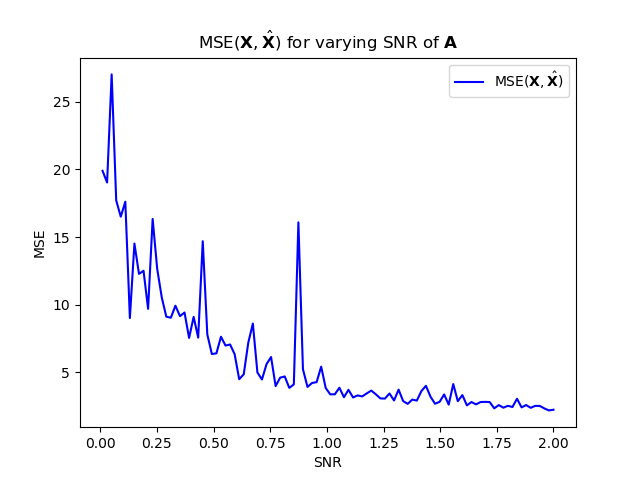
\includegraphics[scale=0.5]{figures/ch_6/X_func_SNR.png}
		\caption{$MSE(\textbf{X},\hat{\textbf{X}})$ estimated from $\textbf{Y}$ specified by $M=6$,$N=k=8$ and $L=1000$, as a function of SNR of given $\textbf{A}$. }
		\label{fig:X_func_SNR}
    \end{minipage} 
    \hfill
    \begin{minipage}[t]{.45\textwidth}
        \centering
		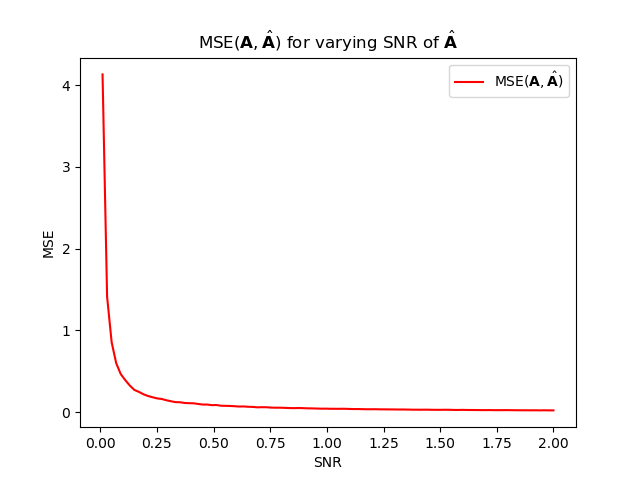
\includegraphics[scale=0.5]{figures/ch_6/A_func_SNR.png}
		\caption{$MSE(\textbf{A},\hat{\textbf{A}})$ where $\hat{\textbf{A}}$ is a function of the SNR. $\hat{\textbf{A}}$ correspond to $\hat{\textbf{A}}$ used in figure \ref{fig:X_func_SNR}}
		\label{fig:A_func_SNR}
    \end{minipage}
\end{figure}  

\subsection{Performance Test of Main Algorithm}\label{sec:Main_test}
In order to evaluate the performance of the main algorithm tests are conducted on several simulated stochastic data sets with different specification. 
The aim is to see how the relationship between $N$ and $M$ affect the performance, in other words how robust the algorithm is towards low density measurements. 
The main algorithm is tested on simulated stochastic data sets specified by $M=8$, $L=1000$, $k=N$ with $N$ in the range $N = [M+1,\dots,36]$, as such $k<\widetilde{M}$ is withhold insuring a solution.
For each value of $N$ ten different data sets are simulated and solved, and the average $\text{MSE}(\mathbf{X}, \hat{\mathbf{X}})$ are used as the result. 
The average $\text{MSE}(\mathbf{X}, \hat{\mathbf{X}})$ are plotted in figure \ref{fig:varyN1}.
\begin{figure}[H]
    \centering
	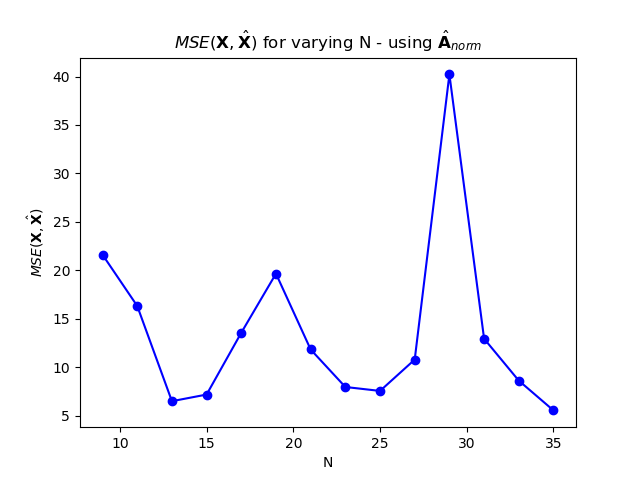
\includegraphics[scale=0.5]{figures/ch_6/varyN1.png}
	\caption{Visualization of $\text{MSE}(\mathbf{X}, \hat{\mathbf{X}})$ of the main algorithm with simulated stochastic data sets specified by $M = 8$, $L=1000$ and $k = N$ for $N = M+1, \hdots , 36$. Average over 10 repetitions for each $N$.}
	\label{fig:varyN1}
\end{figure}
\noindent
From figure \ref{fig:varyN1} it is seen that the $\text{MSE}(\mathbf{X}, \hat{\mathbf{X}})$ lies in the interval $[4,14]$, however no clear trend appears in the plot. 
This suggest that it is not an representative average which have been plotted, thus the test is repeated with more repetitions for value of $N$. The new result of the $\text{MSE}(\mathbf{X}, \hat{\mathbf{X}})$ is seen in figure \ref{fig:varyN2}.
\begin{figure}[H]
    \centering
	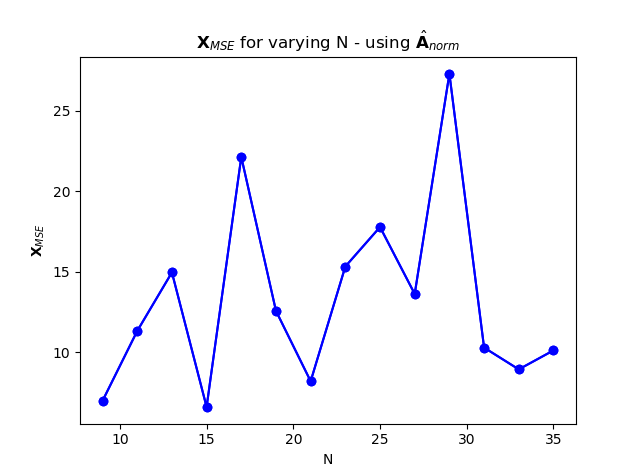
\includegraphics[scale=0.5]{figures/ch_6/varyN2.png}
	\caption{Visualization of $\text{MSE}(\mathbf{X}, \hat{\mathbf{X}})$ of the main algorithm with simulated stochastic data sets specified by $M = 8$, $L=1000$ and $k = N$ for $N = M+1, \hdots , 36$. Average over 500 repetitions for each $N$.}
	\label{fig:varyN2}
\end{figure}  
\noindent
Figure \ref{fig:varyN2} confirms the result of the first test. Thus it must be that average behaviour which is seen. 
This suggest that the performance of the main algorithm is not affected by the relation between $M$ and $N$.
However, this assumption is counter intuitive and it is a contradiction to the results seen in figure \ref{fig:AR1} and \ref{fig:AR2}, where the true $\mathbf{A}$ was utilised. 
Thus the choice of the alternative estimate $\hat{\mathbf{A}}_{\text{norm}}$ might have influenced the results negatively.  
Furthermore it is worth to notice the relative large interval of the $\text{MSE}(\mathbf{X}, \hat{\mathbf{X}})$ suggesting a vary high variance within the resulting $\text{MSE}(\mathbf{X}, \hat{\mathbf{X}})$, which add a certain unreliability to the results \todo{Ændre title i figurerne -- til norm2 of 'MSE' i yakse}.    

\section{Conclusion}
Through this chapter the implementation process has been described, followed by verification tests of the two main elements of the baseline algorithm, respectively the COV-DL algorithm and the M-SBL algorithm. 
From the test of M-SBL on stochastic data sets it was verified that the algorithm provide the expected output and from $\textbf{X}_{MSE}$, and the corresponding visual comparison, the estimate was found to be sufficient. 
The verification of M-SBL was conditioned on the true mixing matrix $\textbf{A}$ as input, to not let the precision of the estimate $\hat{\textbf{A}}$ affect the results.  
Furthermore the possibilities of letting $k = N$ was discussed. Either $N$ nor $k$ is known in practise, but one has to provide the best guess for both $N$ and $k$ to the algorithm in order to provide corresponding number of source signals. By letting $k=N$ one only has to guess the maximal number of active sources and not the relation between active and non active sources, which is considered easier.  
Considering the consequences within the M-SBL, letting $k=N$ will reduce the chance of dislocation, which is seen as an advantage. Furthermore test on the deterministic data confirmed that the estimated active sources was not degraded. Thus it is confirmed that letting $k = N$ is sufficient, and will be used when test the algorithm on real EEG measurements.               

From the verification test of COV-DL, providing the estimate $\hat{\textbf{A}}$, it was that COV-DL did not manage to provide a sufficient result. 
Is was confirmed that the COV-DL resulted in the expected output relative to the implementation, but the output did not comply with the theoretically expected result. 
Thus it is concluded that the theory provided by source \cite[phd2015] was misinterpreted, suggesting partly that the degree of reproducibility of the paper have not been sufficient. 
Due to the time scope of the thesis this issue is not investigated further. 
However, as the estimate of $\textbf{A}$ resulting from COV-DL is crucial in order to estimate the sources signal from real EEG data, it was chosen that the best possible alternative to original estimate must be used, in order to pursue the remaining elements of the thesis. Then, the missing estimate must be taking into account when evaluating the final results.
Different suggestions for an alternative estimate of $\textbf{A}$ was proposed an evaluated by the resulting $\textbf{X}_{MSE}$. Here the it was found that fixed estimated $\hat{\textbf{A}}_{norm}$ generated from a normal distribution with mean $= 0$ and variance $=2$ provided the best result, when tested on stochastic data sets resembling real EEG measurements.          
      
Lastly the performance of the final baseline algorithm was tested on stochastic data sets. Here tests were performed on varying N in order to investigate performance relative to the relation between M and N. For each value of N repetitions was conducted and the average $\textbf{X}_{MSE}$ was evaluated. The $\textbf{X}_{MSE}$ was found to lie within an interval from 2 to 25, without any characteristic trend relative to the increasing N. From this is it concluded that the performance do not rely on the relation between N and M. Despite that this was indicated by the tests where the true $\textbf{A}$ was utilised. 
Thus the lack of a precise estimate of $\textbf{A}$ might influence the final results. 

Overall, the implementation of the baseline algorithm is approved. However the performance is not as good as expected. From this the baseline algorithm is ready  to be tested on real EEG measurements in order to evaluated the performance with respect to the problem statement of this thesis. This test is specified and conducted in the next chapter.           



